\documentclass[12pt]{article}
% This first part of the file is called the PREAMBLE. It includes
% customizations and command definitions. The preamble is everything
% between \documentclass and \begin{document}.

\usepackage[margin=1in]{geometry}  % set the margins to 1in on all sides
\usepackage{graphicx}              % to include figures
\usepackage{amsmath}               % great math stuff
\usepackage{amsfonts}              % for blackboard bold, etc
\usepackage{amsthm}                % better theorem environments

\usepackage{rotating} % for sideway table
\usepackage{xcolor}
\usepackage{hyperref}
\hypersetup{
    colorlinks,
    linkcolor={red!50!black},
    citecolor={blue!50!black},
    urlcolor={blue!80!black}
}
\usepackage{cleveref}

\usepackage{array,tabularx}

\newenvironment{conditions*}
  {\par\vspace{\abovedisplayskip}\noindent
   \tabularx{\columnwidth}{>{$}l<{$} @{${}={}$} >{\raggedright\arraybackslash}X}}
  {\endtabularx\par\vspace{\belowdisplayskip}}
  
\usepackage{float}
\restylefloat{table}

% various theorems, numbered by section

\newtheorem{thm}{Theorem}[section]
\newtheorem{lem}[thm]{Lemma}
\newtheorem{prop}[thm]{Proposition}
\newtheorem{cor}[thm]{Corollary}
\newtheorem{conj}[thm]{Conjecture}

\DeclareMathOperator{\id}{id}

\newcommand{\bd}[1]{\mathbf{#1}}  % for bolding symbols
\newcommand{\RR}{\mathbb{R}}      % for Real numbers
\newcommand{\ZZ}{\mathbb{Z}}      % for Integers
\newcommand{\col}[1]{\left[\begin{matrix} #1 \end{matrix} \right]}
\newcommand{\comb}[2]{\binom{#1^2 + #2^2}{#1+#2}}

% bibliography
\usepackage{natbib}
\bibpunct{(}{)}{;}{a}{}{,} % no comma between author and year

\title{Paper title}
\author{Anh Le}


\begin{document}
\maketitle

\section{Puzzle: FDI does not lead to development}

In recent decades, foreign direct investment (FDI) global flow has steadily increased, rising to over \$1.5 trillion dollars in 2014. For developing countries, FDI flow is also remarkably robust to global downturn (\Cref{fig:globalfdi}). Moreover, FDI is important not only because of its volume, but also because it has been enthusiastically advocated by major international organizations as a key factor to economic development.\footnote{http://www.imf.org/external/pubs/ft/fandd/1999/03/mallampa.htm, http://www.weforum.org/reports/foreign-direct-investment-key-driver-trade-growth-and-prosperity-case-multilateral-agreement} This assumption is also shared widely within political science, where much of the literature starts with the assumption that countries want to seek FDI for its many benefits. The question that these works focus on is \textit{how} countries can attract FDI, not \textit{whether} they want to do so \citep{Jensen2003, Li2003, Li2006, Ahlquist2006}.\footnote{Two recent exceptions are \citet{Pinto2013, Pandya2013}, which are the first to investigate the demand for FDI.} 

\begin{figure}[!ht]
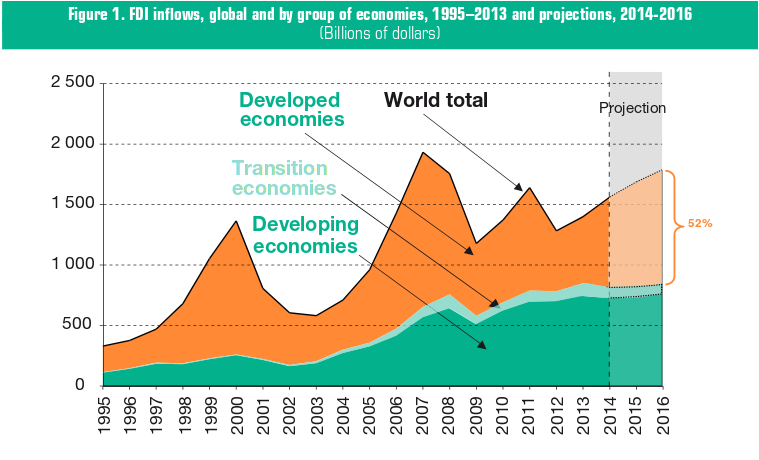
\includegraphics[width=\textwidth, height=\textheight,keepaspectratio]{../figure/global_fdi}
\caption{Source: World Investment Report, 2014}
\label{fig:globalfdi}
\end{figure}

Underlying this mode of thinking is the assumption that FDI various benefits to developing countries, such as capital and employment. However, the most important promise that FDI holds to growth is the spillover of productivity between the foreign firms and the domestic firms. This can happen if local firms hire workers that were trained in a foreign firms, improve productivity through backward and forward linkage with foreign firms, or imitate foreign technology. According to growth theory, it is FDI's spillover, not capital or employment, that serves as a major channel for the technological innovation that is a requisite for economic growth \citep{Findlay1978}. In this view, spillover from FDI is also public good, providing benefits to the local firms in ways that the foreign firms do not take into account in their private calculations. This provides the justification for countries' giving investment incentives to FDI firms in order to rectify the undersupply of FDI, closing the gap between private and social returns. 

And yet, there is no conclusive evidence of FDI having a positive effect on growth \citep{Nair-Reichert2001, Carkovic2002} or poverty reduction \citep{Guerra2009} (\Cref{fig:fdipoverty}). A substantial literature has developed to explain this puzzle, concluding that the growth-enhancing and spillover effect of FDI is conditional on absorptive capacity of local firms. Crossnationally, scholars find that positive growth effect of FDI is more likely when the technological gap between the local and foreign firms are small \citep{Nunnenkamp2004}, and when host countries have strong financial and institutional development \citep{ Durham2004}. Similarly, absorptive capacity, measured by the level of schooling in host economy, conditions the transfer of technology between foreign and local firms across regions in China \citep{Fu2008} and countries in Latin America \citep{Willem2004}.

\begin{figure}[!ht]
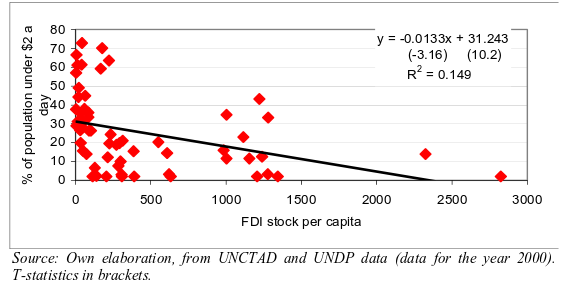
\includegraphics[width=\textwidth, height=\textheight,keepaspectratio]{../figure/fdi_poverty}
\caption{Relationship between FDI and poverty}
\label{fig:fdipoverty}
\end{figure}

Despite this resounding conclusion that the effect of FDI is highly conditional and that investment incentives do not work, why do countries still fixate so much on bringing in FDI instead of developing the local absorptive capacity \citep{Blomstrom2002}? For example, Ireland provided foreign investors with lower tax rate, lower land price, and cash grants for R\&D that do not need to be repaid. China also used a tax holiday (two years of no tax and three year of half the normal tax rate) in their special economic zones to attract more foreign firms \citep{Telford2001}. We see the same widespread use of investment incentives in Southeast Asia \citep{Fletcher2002}. In Vietnam, the race to offer incentives to foreign firms rages on even among sub-national units, where provincial governments defied the central government's directive and offered extra-legal incentives to FDI firms \citep{Vu2007}. Not only do these measures not work, they also deprive countries of revenues that could be spent on improving the local labor quality and investment climate, which are much more conducive to spillover effect and growth.

My dissertation project focuses on this empirical puzzle: if the positive effect of FDI is uncertain, why is there so much focus on attracting it even at the expense of generating revenues?\footnote{Countries lose revenue not only through offering financial incentives but also because FDI firms can easily dodge corporate income tax with transfer pricing \citep{Bartelsman2003}.} If developing absorptive capacity is so crucial to making FDI growth-enhancing, why is it often neglected? To understand this puzzle, I propose that we need to take incorporate the calculus of the individual bureaucrat and government officials, who may be more interested in the potential rents from foreign firms than the spillover and growth-enhancing effect of FDI. This is a potential reason why we often see countries (i.e. government officials) being so enthusiastic about attracting FDI, yet not so passionate about developing the local capacity that enables FDI to actually have a positive effect on growth. Both the empirical puzzle and the hypothesis have not been considered by scholars in political economy.

\begin{figure}[!ht]
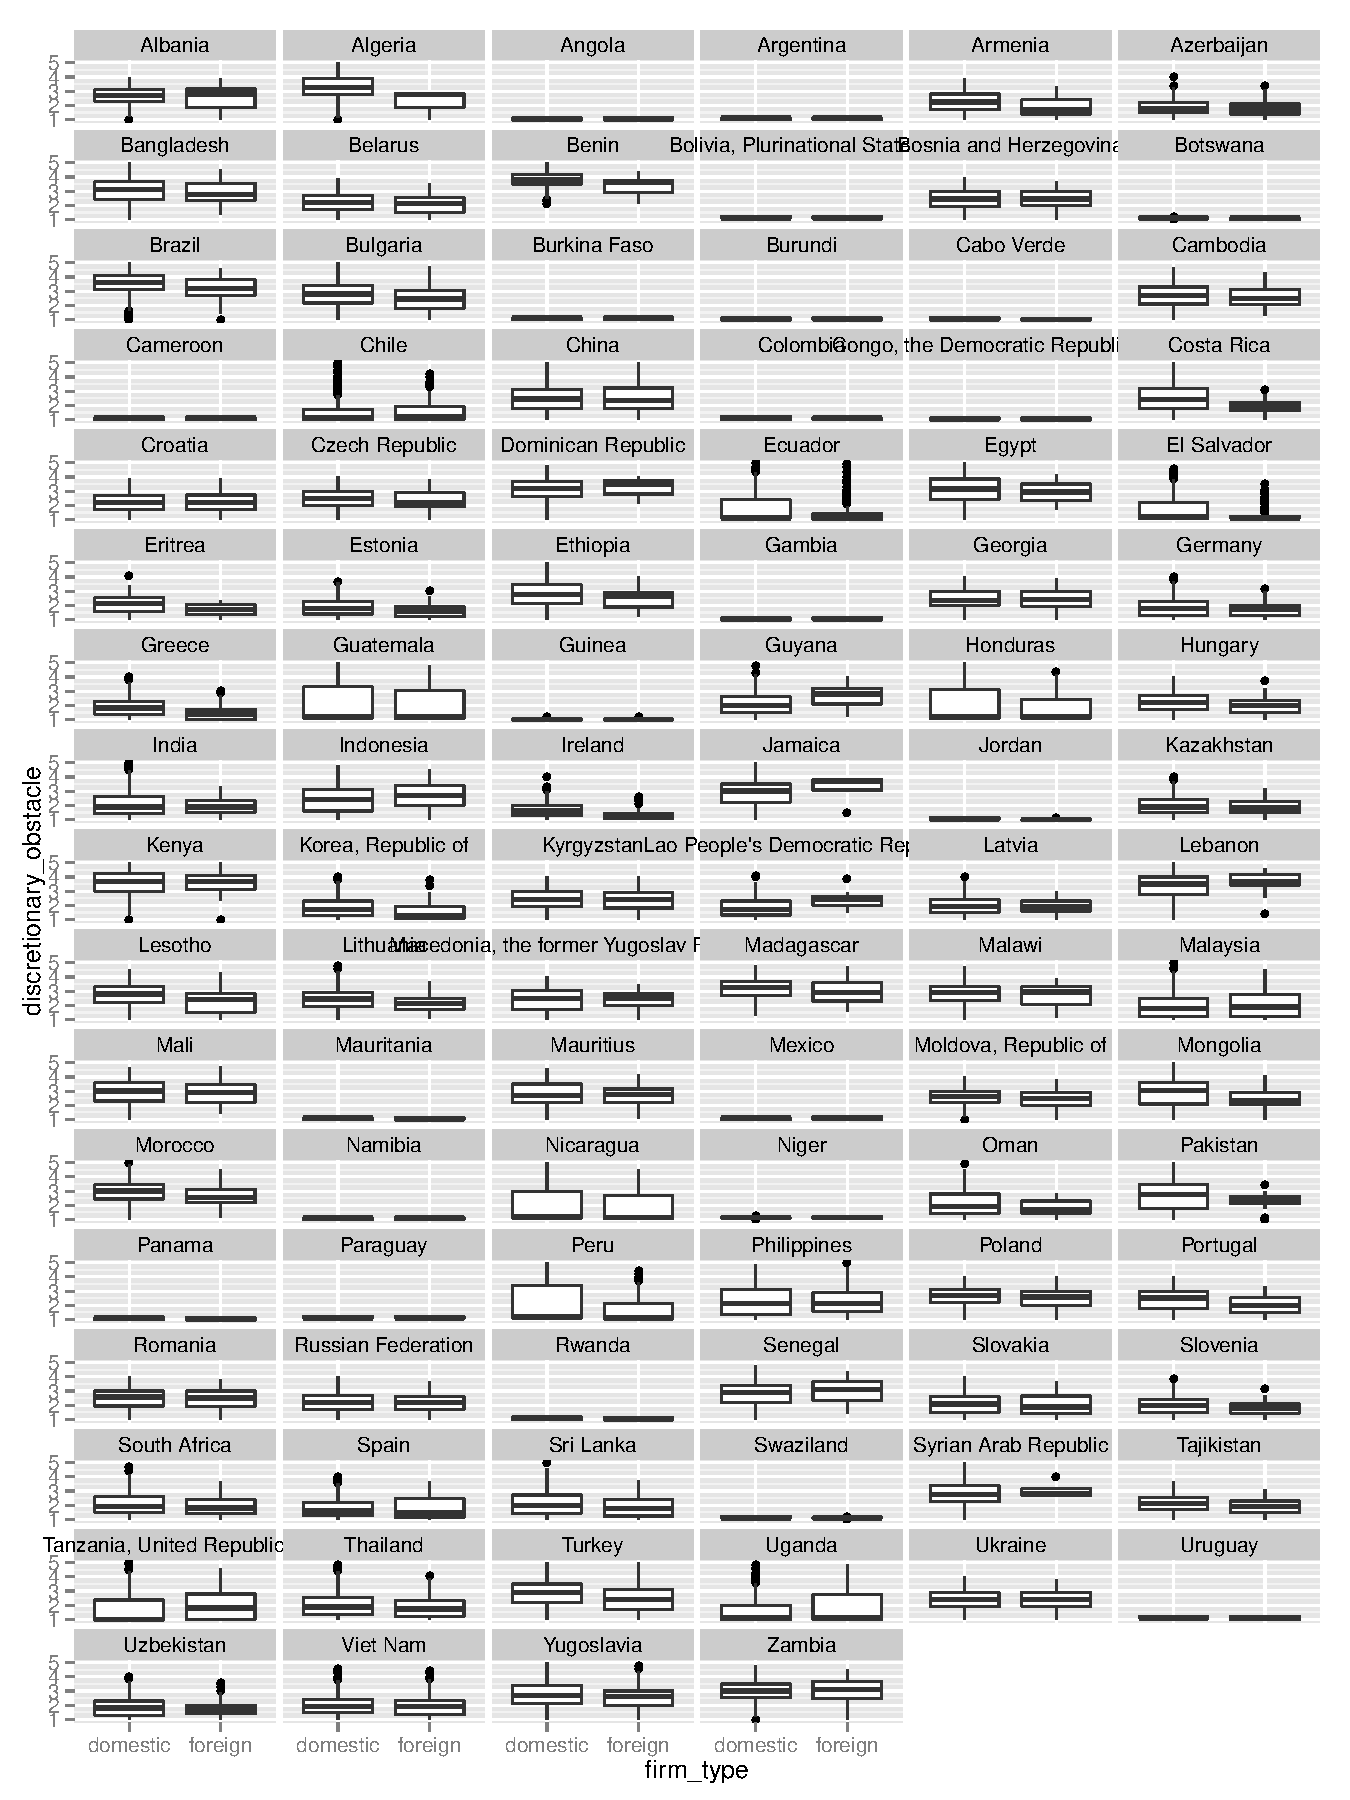
\includegraphics[width=\textwidth, height=\textheight,keepaspectratio]{../figure/fdi_domestic_treatment}
\caption{The treatment of FDI and domestic firms}
\label{fig:fdi_domestic_treatment}
\end{figure}

This study looks at the interesting phenomenon of FDI engaging in corruption, something that the literature is un-equipped to deal with (except Malesky). It also looks at the issue of private sector development politically, having important welfare and social impact here.


\section{Theory}

Government policy is important in inducing spillover.

Spillover can happened in different ways: competition (unless the incoming firm is granted monopoly status) similar to how arm's length trade put pressure on domestic firms to reduce inefficiency \citep{Glass2002}, imitation (both reverse engineering and copying managerial techniques, reverse engineering deserve government support) \citep{Wang1992}, human capital spillover of workers in foreign firms moving to domestic firms (Czech firms) \citep{Djankov2000}, technology transfer. Export demonstration, because exports often involve high fixed cost to set up a distribution and transport infrastructure, learn about foreign taste and regulatory framework. Domestic firms can learn from foreign firms about how to export, and exporting firms are more productive \citep{Aitken1997}.

Corruption: \citep{Malesky2015} is about foreign firms bribe to get into high profitability and protected sectors. Mine is about the calculus of the officials and its effect on the private domestic sector


\section{Hypothesis: Rent seeking}

- corruption literature
- local central literature

Political decentralization increases bribery \citep{Fan2009}. Uncoordinated corruption, more tiers of governments, increase corruption.

Fiscal decentralization reduces corruption \citep{Guerra2009}

\section{Research design}

Hypothesis: In sectors / countries where there is a lot of corruption between the politicians and FDI, there will be less private sector development.

- corruption between the politicians and FDI: 

+ Vietnam case: 1) sectors with protection against FDI (group A) 

+ Vietnam + crossnational: 2) sectors with natural monopoly / high degree of profitability. Natural monopoly / profitability = access is more valuable means more incentive to bribe, small numbers of firms means easier coordination. (But why wouldn't the bureaucrat want to collude with the domestic firms instead? Perhaps because there are no big enough domestic firms. We can control for this by pre-FDI private sector)


- private sector development = measured on discretionary treatment measure (time deal with officials, officials' attitude, tax rate), not so much on infrastructure

\subsection{Crossnational}

Countries with a lot of corruption + a lot of FDI will see larger gap between the treatment of FDI and domestic firms.

Corruption alone is not enough. FDI alone is not enough.

What about corruption reducing FDI? Is there a sample of countries with high FDI and high corruption? (a graph would be neat)

INSERT GRAPH HERE


\subsection{Provincial leader vs central}

\citep{Malesky2008} Straight ahead on red -- central incentive is growth

\citep{Sheng2007} China's central government exert more control over provinces that has high FDI (through party organization channel)

\subsection{Sectoral}

\citep{Malesky2015} discusses how foreign firms in Group A restricted industries have to pay more bribes (telecommunications, radio and TV broadcasting, transportation, and distribution). We can use this as a measure of FDI corruption, especially since some of the restrictions applies to foreign firms only.


\subsection{Conjoint analysis}



- Selection bias (if a countries disriminated against FDI, then the surveyed firms are already more capable)


% http://zunia.org/sites/default/files/media/node-files/04/155466_04050041.pdf

Foreign firms often face fewer obstacles

Asia crowding in (SK, Thailand, pakistan), Latin America crowd out (crowdin or crowdout). Paper does not discuss the policy nor the motivation

Colombia, Mexico, Hong Kong, Indonesia, and Taiwan

Argentina, Brazil,Colombia, Korea, Malaysia, Thailand in Asia

Evidence is mixed across regions / countries DOES FOREIGN DIRECT INVESTMENT PROMOTE ECONOMIC GROWTH? EVIDENCE FROM EAST ASIA AND LATIN AMERICA 

in Latin America, high corruption = high FDI http://www.ccsenet.org/journal/index.php/jms/article/viewFile/32108/18686

http://www.nytimes.com/2012/04/22/business/at-wal-mart-in-mexico-a-bribe-inquiry-silenced.html?pagewanted=all (Walmart bribe in Mexico)

\clearpage
\bibliographystyle{chicago}
\bibliography{library}
\end{document}
